\chapter{Performance Evaluation}
\label{Chapter5}
\lhead{Chapter 5. \emph{Performance Evaluation}} % Write in your own chapter title to set the page header

In this chapter, we first will introduce our designed performance metrics in order to properly evaluate our proposed adaptive fanout \pp ~\gp. Then we will explain our simulation environment settings. Finally, we will analyze the simulation results.

\section{Performance Metrics} \label{pm}
As we stated in Section \ref{basic gossip}, the objective of our proposed approach is to achieve the balance between fast broadcasting time and long network lifetime. So obviously, the first two performance metrics that we proposed are \emph{Average \nl} and \emph{Average Message Broadcast Time}. Other performance metrics are \emph{Average Overhead Per Node Per Message}, \emph{Average Consumed Energy Per Node Per Message}, and \emph{Average Number of Success Broadcast Messages}.

\subsection{Average Network Lifetime}
%\textbf{Average Network Lifetime}

Before we define \emph{Average Network Lifetime}, we need to define \emph{Network Lifetime} first. 

\textbf{Network Lifetime}: The time duration which a wireless ad-hoc network can physically broadcast \msgs ~successfully.

When a \gn's energy is depleted, this \gn ~will no longer be able to transmit and receive new broadcast \msgs. Thus, this network is considered to be physically unable to broadcast \msgs ~successfully. Now the definition of \emph{Average Network Lifetime} is simply just an average over all \emph{Network Lifetime} under $n$ \gns ~case. For example, if we ran $s$ simulations under $n=10$ setting, and we denote \emph{Average Network Lifetime} for $10$ \gns ~as $L_{avg\_10}$, then the following equation can be used to calculate the \emph{Average Network Lifetime}.

\[ L_{avg\_10} =\frac{L_1 + L_2 + \ldots + L_{s}}{s} \]

This performance metric measures how long a wireless ad-hoc network with $n$ \gns ~can stay connected when running our proposed adaptive fanout \gp.

\subsection{Average Message Broadcast Time}
%\textbf{Average Message Broadcast Time}

Before we jump into the definition of \emph{Average Message Broadcast Time}, we first need to clearly define \emph{Message Broadcast Time}.

\textbf{Message Broadcast Time}: The maximum delay among \gns ~for each broadcast \msg.

Because here we are trying to measure the broadcast time of a certain \msg, it only makes sense when we sample the maximum delay among all \gns ~because the \msg ~received time of the last \gn ~determined our message broadcast time for a particular \msg. Now the \emph{Average Message Broadcast Time} is just an average over all \msg ~broadcast time under $n$ \gn ~case. Now because the randomness of our proposed \gp, each simulation under $n$ \gn ~case can result in different number of success broadcast \msgs. Therefore, for $n$ \gn ~case simulations, we first calculate the \emph{Average message broadcast time} for each simulation. And then we perform the average among those number to obtain this performance metrics data.

For example, let's denote the \emph{Average Message Broadcast Time} for $i$th simulation as $T_i$ and the \emph{Average Message Broadcast Time} for $n$ nodes as $T_{avg\_n}$. If we performed $s$ simulations, then the following equation can be used to calculate this metric:

\[ T_{avg\_n} = \frac{T_1 + T_2 + \ldots + T_s}{s} \]

This metric indicates the time needed for a broadcast \msg ~to reach every \gn ~in the network.

\subsection{Average Overhead Per Node Per Message}

The \emph{overhead} here is defined as the total number of packets sent by a \gn. These packets includes Ack packet, Request packet, and Data packet. For every simulation, in order to accurately measure the overhead for each \gn ~and for each broadcast \msg, we simply performed an average over $n$. And then take that number and further average over number of broadcast \msgs being sent. So for $k$th simulation, if we denote the overhead of node $i$ for \msg ~$j$ as $O_{ij}$, the number of \gns ~are $n$, and the system broadcast $m$ \msgs. Then for this simulation, the \emph{Average Overhead Per Node Per Message} can be computed using the following equation:

\[ O_{k} = \frac{(O_{11} + O_{21} + \ldots + O_{n1})  + \ldots + (O_{1m} + O_{2m} + \ldots + O_{nm})}{n\times m} \]

If we performed $s$ simulations under $n$ \gns ~setting, then the \emph{Average Overhead Per Node Per Message} among these simulations is:

\[ O_{avg\_n} = \frac{O_1 + O_2 + \ldots + O_s}{s} \]

%+ (O_{12} + O_{22} + \ldots + O_{n2})
%\mbox{Average Overhead Per Node Per Message}

This performance metric indicates how many packets are sent out for a \gn ~to facilitate broadcasting one \msg. 

\subsection{Average Energy Consumption Per Node Per Message}

This performance metric is quite self-explanatory. We measure the amount of energy consumed by each \gn ~during the simulation. For each simulation, first we average among every \gn's energy consumption. Then we take that number and average among $m$ \msgs. If we denote $E_k$ as the \emph{Average Energy Consumption Per Node Per Message} for the $k$th simulation under $n$ \gns. Then 

\[ E_k = \frac{E_{node\_1} + E_{node\_2} + \ldots + E_{node\_n}}{n\times m} \]

Now if we ran $s$ simulations, then \emph{Average Energy Consumption Per Node Per Message} under $n$ \gns ~can be calculated using the following equation:

\[ E_{avg\_n} = \frac{E_1 + E_2 + \ldots + E_s}{s} \]

This metric measures the amount of energy needed for a \gn ~to facilitate broadcasting one \msg. 

\subsection{Average Number of Broadcast Messages}

This metric measures how many \msgs ~can be successfully broadcast with limited energy sources. If we ran $s$ simulations under $n$ \gns ~setting, this metric can be computed using the following equation:

\[ N_{avg\_n} = \frac{N_1 + N_2 + \dots + N_s}{s} \]

\section{Simulation Environment Settings}

In order to properly evaluate our proposed \pp ~\gp, we need to compare it to the same basic \pp ~\gp ~but with constant \emph{Fanout} settings. Here we picked three typical \emph{Fanout} values. They are $f=1, 5, 10$. By obtaining performance metrics data from these three constant fanout settings, we can study how different \emph{Fanout} affect protocol performance. 

The simulation environment setting is summarized below.

\begin{itemize}
	\item Fanout: 1, 5, 10, or adaptive
	\item Number of nodes: 10, 50, 90, 130, 170
	\item \wf ~speed among \gns: 1Mbps
	\item \wf ~speed between the \sn ~and a \gn: 11Mbps
	\item MAC: IEEE 802.11 for \gns ~and \sn
	\item RTS/CTS: On
	\item Gossip node maximum \wf ~range: 50m
	\item Source node maximum \wf ~range: 500m
	\item Simulation stop time: 100000.0s
	\item Initial battery energy: 108.0J  (3V)
	\item Gossip interval: 1.0s
	\item Request interval 5.0s
	\item \wf ~radio idle current: 0.0A
	\item \wf ~radio sleep current: 0.0A
	\item \wf ~radio transmit current: 0.38A
	\item \wf ~radio receive current: 0.313A
	\item Gossip nodes IP address: 10.1.1.0/24
	\item Source node and a \gn's IP address: 10.1.2.0/24	
\end{itemize}

As we stated earlier, the simulation stop time is set to be large enough so that the energy sources on \gns ~will be depleted first. Thus, it will trigger the termination of our simulations. 

\section{Results Analysis}

In order to obtain simulation data for these $f=1,5,10, adaptive$ settings, we ran 100 simulations for each number of \gns ~setting. Because of the random placement of \gns ~can potentially generate a disconnected topology, some of the simulations will be terminated in the beginning. Table \ref{table:sim} shows the number of successful simulations under each number of \gns ~setting. It is worth noting that this table holds true for all four \emph{Fanout} settings.

\begin{table}[h]
	\centering
	\caption{Number of Simulations Run}
	\label{table:sim}
	\begin{tabular}{|c|c|c|}
		\hline 
		Number of gossip nodes & Total number of simulations & Number of success simulations \\ 
		\hline 
		10 & 100 & 85 \\ 
		\hline 
		50 & 100 & 52 \\ 
		\hline 
		90 & 100 & 50 \\ 
		\hline 
		130 & 100 & 46 \\ 
		\hline 
		170 & 100 & 34 \\ 
		\hline 
	\end{tabular} 
\end{table}

By conducting statistical analysis based on the method in Section \ref{pm}, we were able to extract the data of each performance metrics. 

Figure \ref{fig:brTime} depicts the \emph{Average Message Broadcast Time} over number of \gns. As we would expect, under any \emph{Fanout} setting, the \emph{\ambt} will increase as the number of \gns ~increase. It is especially obvious for $f=1$ setting. For other \emph{Fanout} settings, their \emph{\ambt} are much shorter than $f=1$ setting across different number of \gns ~settings. We can see a huge performance improvement when \emph{Fanout} is switched from 1 to 5. That is because a \gn ~can forward the broadcast \msg ~to more neighbors comparing to $f=1$ setting. However, the performance improvement from $f=5$ to $f=10$ is marginal. We believe that it is related to the average node's degree since a \emph{Fanout} setting that exceeds the number of neighbors a \gn ~has will bring no additional performance boost. Our adaptive fanout approach performed as good as $f=5$ setting even though its \emph{Fanout} is ranging from 1 to 5 during a simulation. 

\begin{figure} 
	\centering
	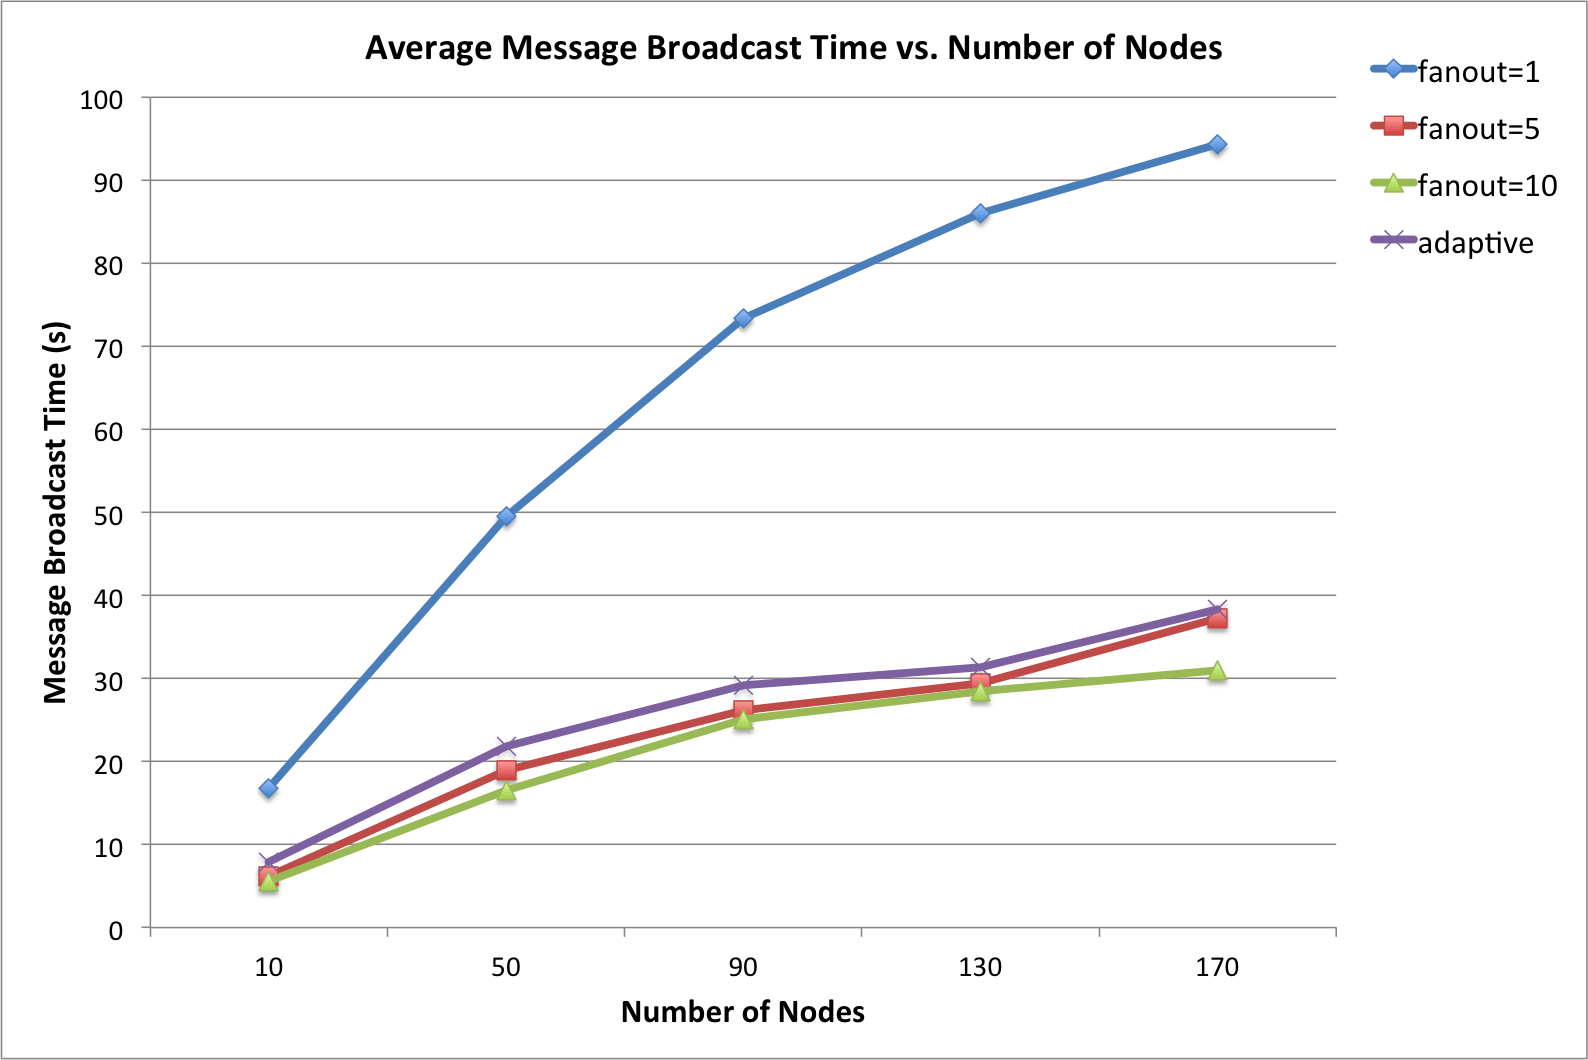
\includegraphics[width=5.5in]{brTime.png}
	\caption{Average message broadcast time vs. number of nodes}
	\label{fig:brTime}
\end{figure}

Figure \ref{fig:life} presents the \emph{Average Network Lifetime} over different number of \gns. For three constant \emph{Fanout} settings, the \emph{\anl} decreases as \emph{Fanout} increases. This is within our expectation because for every gossip round, a \gn ~with a higher \emph{Fanout} setting will have to contact more neighbors thus consume more energy. $f=1$ setting has the best \emph{\anl} but as we see in Figure \ref{fig:brTime}, it has the worst \emph{\ambt}. Under $f=5$ setting, the \emph{\anl} is reasonably good while the \emph{\ambt} is shorter. However, our proposed adaptive fanout setting can achieve even better \emph{\anl} comparing to $f=5,10$ settings while still perform as good as the other two in terms of \emph{\ambt}. 

\begin{figure} 
	\centering
	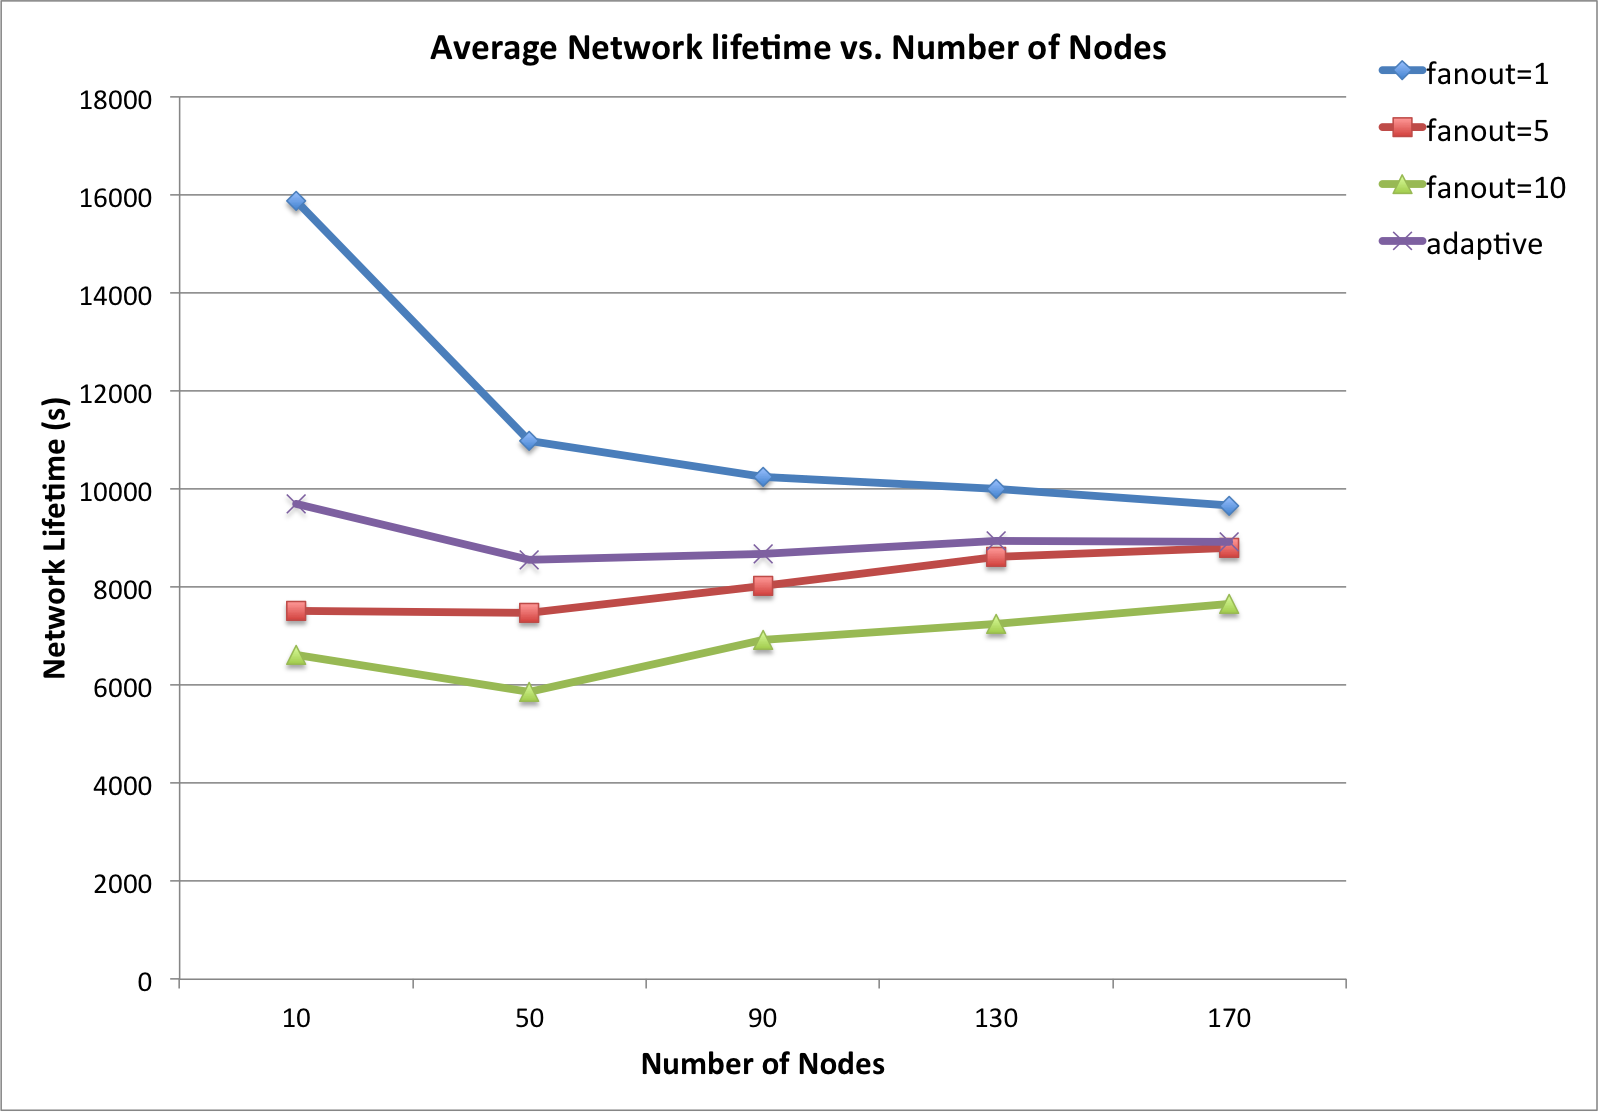
\includegraphics[width=5.5in]{life.png}
	\caption{Average network lifetime vs. number of nodes}
	\label{fig:life}
\end{figure}

From Figure \ref{fig:energy}, we can see that as number of \gns ~increases, the \emph{Average Energy Consumption Per Node Per Message} increases as expected. For the ease of discussion, in the following chapter we will call it \emph{Average Energy Consumption}. The interesting part here we would like to point out is that $f=1$ setting actually has the highest energy consumption. The reason is that even though it has the longest \emph{\anl}, it also has the worst \emph{\ambt}. So given these two constrains, the number of \msgs it can broadcast is less than other \emph{Fanout} settings. Since we computed this metric on a per \msg ~basis, it would result in a higher \emph{\aec}. Under $f=5$ and adaptive fanout setting, their \emph{\aec} plots are almost overlapping each other. The reason is the trade off between \emph{\ambt} and \emph{\anl}. $f=10$ setting has the lowest \emph{\aec} except for 170 \gns ~setting, but as shown in Figure \ref{fig:life}, it has the worst \emph{\anl}. 

\begin{figure} 
	\centering
	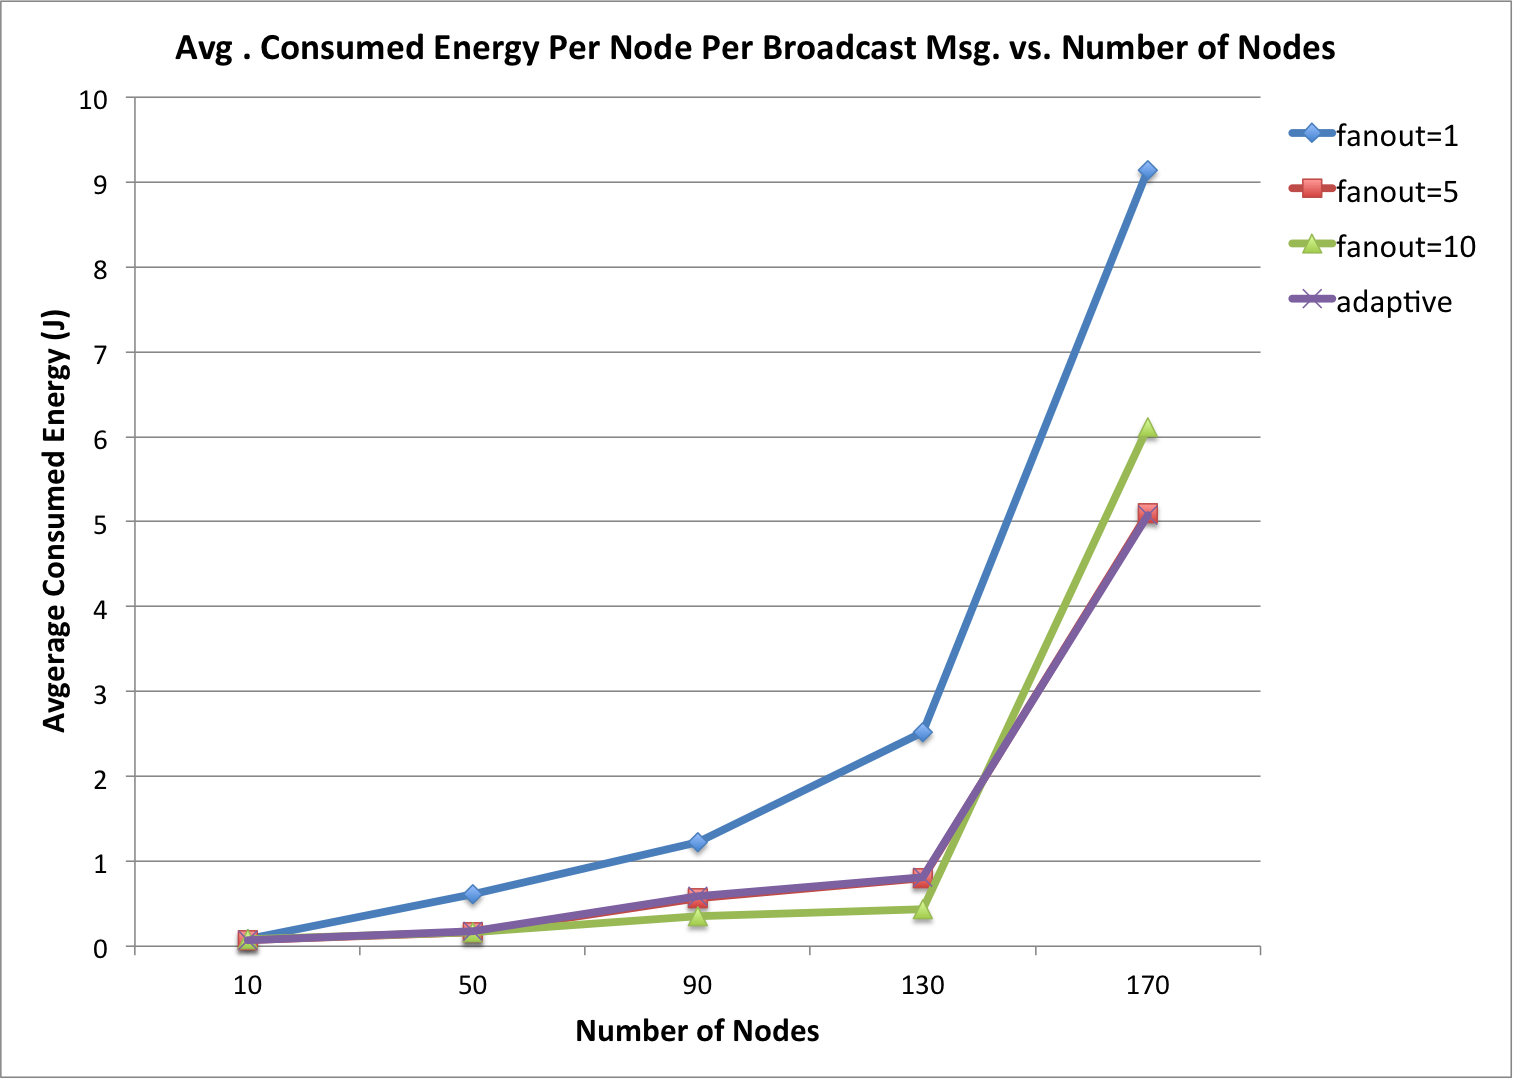
\includegraphics[width=5.5in]{energy.png}
	\caption{Average consumed energy per node per message vs. number of nodes}
	\label{fig:energy}
\end{figure}

Figure \ref{fig:overhead} shows the results of \emph{Average Overhead Per Node Per Message} over various number of \gns. For the ease of discussion, from now on we will call it \emph{\ao}. Comparing Figure \ref{fig:overhead} to Figure \ref{fig:energy}, we can see that the shape of each plot is almost identical even though the unit on the y-axis is different. That is because energy consumption is closely related to overhead since overhead is defined as the number of packets sent by each \gn. Therefore, the same analysis on Figure \ref{fig:energy} can be applied here as well.

\begin{figure} 
	\centering
	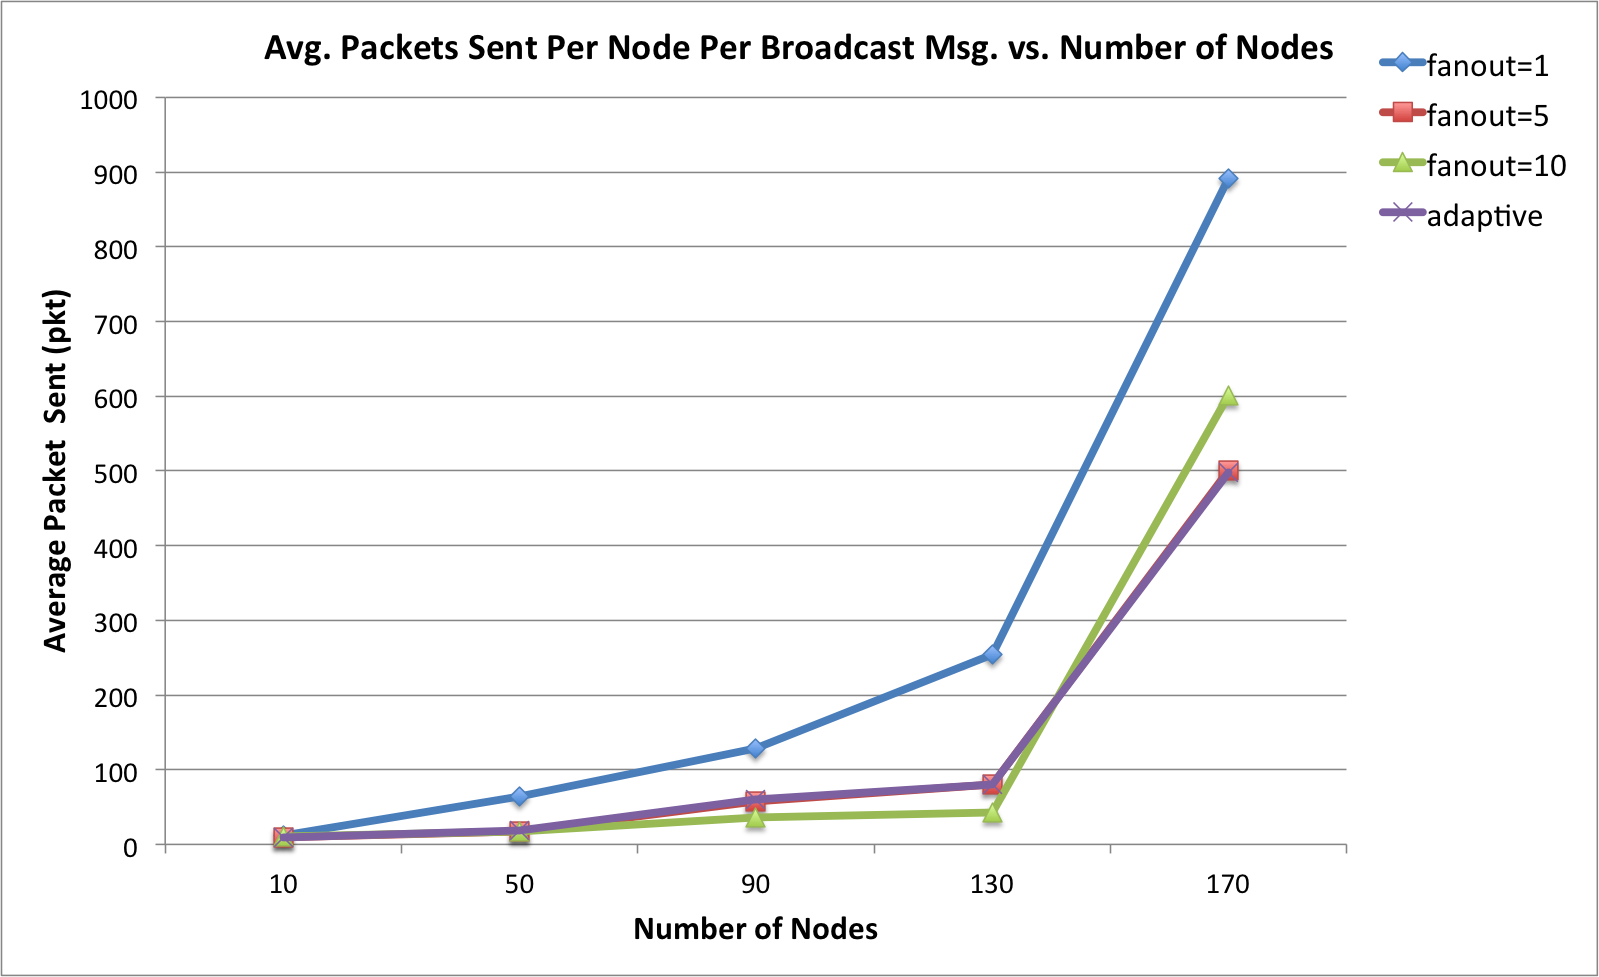
\includegraphics[width=5.5in]{overhead.png}
	\caption{Average overhead per node per message vs. number of nodes}
	\label{fig:overhead}
\end{figure}

Lastly, Figure \ref{fig:brNum} presents the number of \msgs broadcast over different number of \gns. $f=1$ setting can deliver the least amount of \msgs comparing to other \emph{Fanout} settings. In general, higher \emph{Fanout} setting will increase the number of \msgs the protocol can deliver. However, as we see in Figure \ref{fig:brTime}, switching \emph{Fanout} from 5 to 10 would result in a very limited performance boost. Our proposed adaptive fanout approach performed as good as $f=5,10$ setting while as shown in Figure \ref{fig:life} it has longer \emph{\anl}.

\begin{figure} 
	\centering
	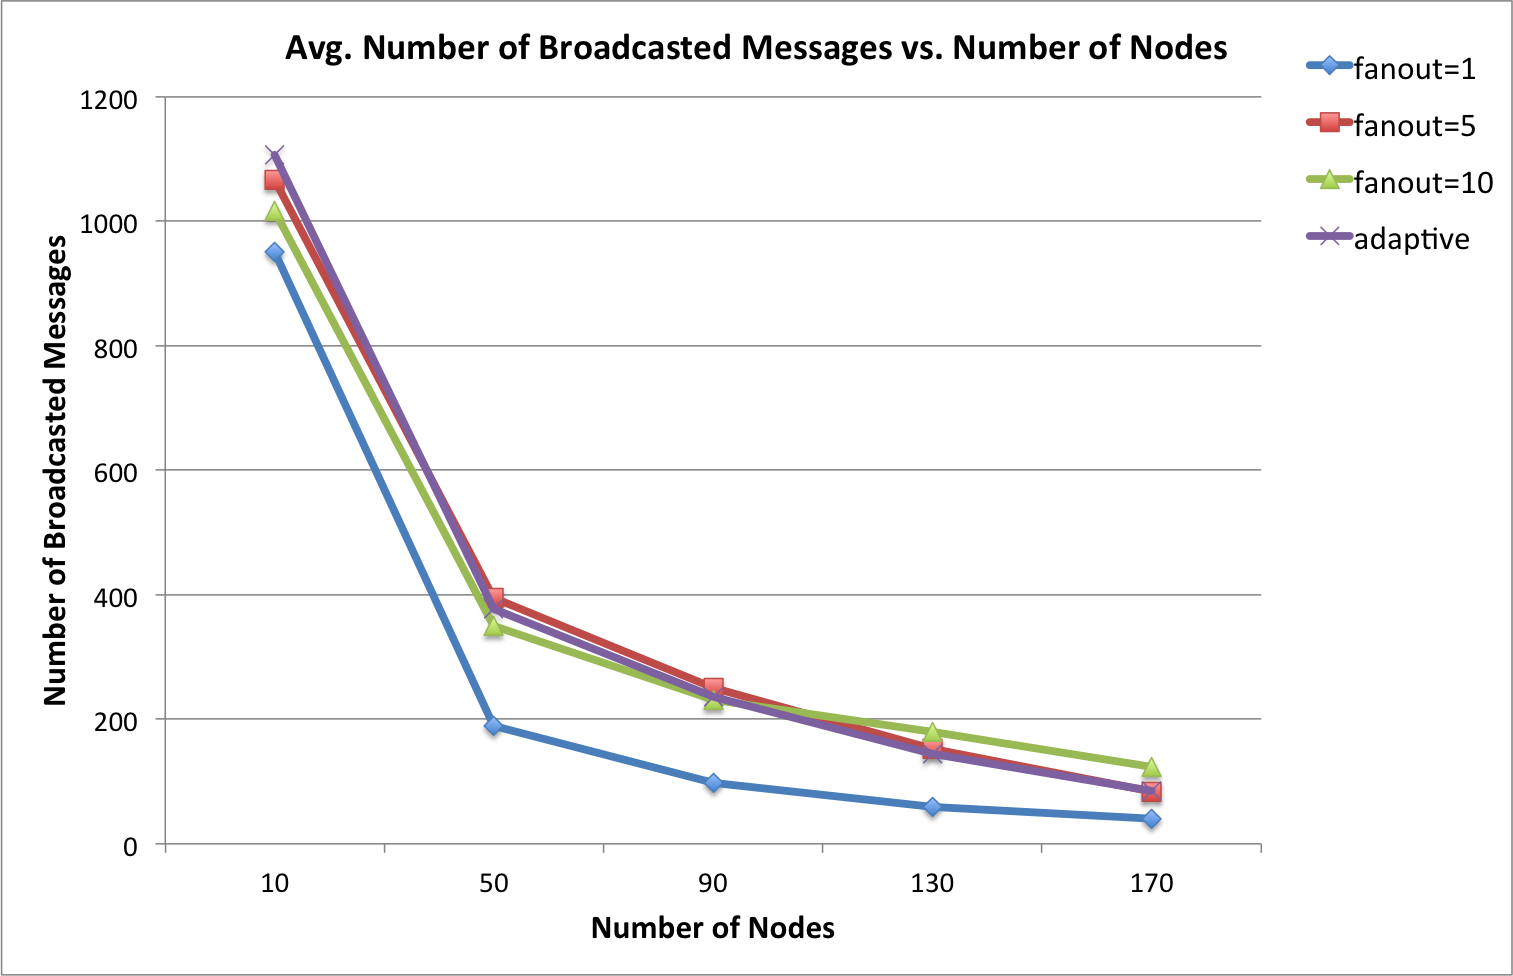
\includegraphics[width=5.5in]{brNum.png}
	\caption{Average number of broadcast messages vs. number of nodes}
	\label{fig:brNum}
\end{figure}